\documentclass[10pt,a4paper]{article}
\usepackage[utf8]{inputenc}
\usepackage{amsmath}
\usepackage{amsfonts}
\usepackage{amssymb}
\usepackage{graphicx}
\usepackage[margin=2cm]{geometry}

\author{Daniel Haehn, Fiona Wood, Sharon Zhou}
\title{CS 279 HW2 Data Analysis}
\begin{document}
\maketitle
\section{Design}
We only removed one data point from our analysis, from an in person user test who was observed to take a break in the middle of their ribbons testing.
\section{Results}
We found that the improvement with commandmaps was significant, but there was not a significant difference between trackpad, trackball, and mouse users. 
\\ \\
The results in R for the paired T test were: 

\texttt{>t.test(data4\$avgclicktimecmdmp, data4\$avgclicktimeribbons, paired=TRUE) \\
Paired t-test \\
data:  data4\$avgclicktimecmdmp and data4\$avgclicktimeribbons \\
t = -9.1619, df = 70, p-value = 1.336e-13 \\
alternative hypothesis: true difference in means is not equal to 0 \\
95 percent confidence interval: \\
 -724.4809 -465.4468 \\
sample estimates: \\
mean of the differences \\
              -594.9639 }
\\ \\ \\
The ANOVA between-subjects test showed the results were device-independent.

\texttt{>res = ezANOVA(data=stacked\_data, dv=avgclicktime, wid=user, within=which, between=.(dev))\\
res\\
\$ANOVA \\
     Effect DFn DFd          F            p p<.05         ges \\
2       dev   2  68  0.1426021 8.673576e-01       0.003102044 \\
3     which   1  68 88.6188769 6.077302e-14     * 0.251693247 \\
4 dev:which   2  68  2.9509884 5.901972e-02       0.021909980}
\\ \\ \\

The histogram of the average difference for each user between time spent completing CommandMaps and Ribbons is shown below.

\begin{figure}
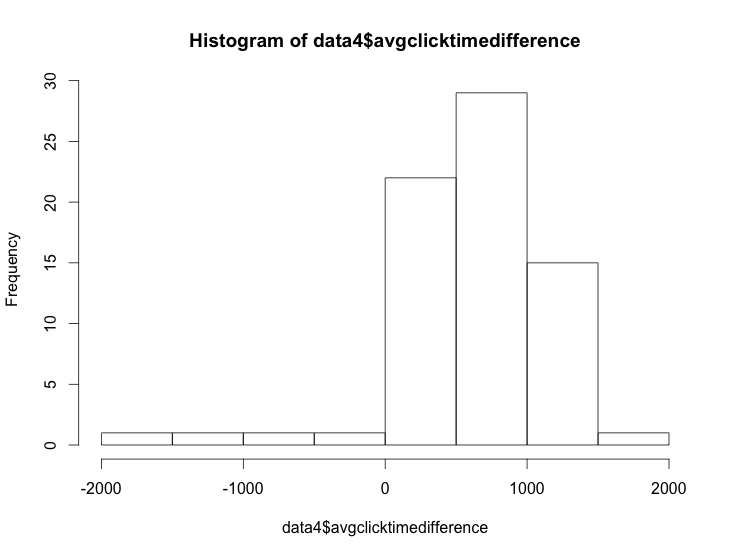
\includegraphics[width=\linewidth]{avgclicktimediff.png} 
\caption{Click time differences}
\end{figure}


\section{Discussion}
There were no significant differences between lab-based and online data. In fact, the only outlier we were sure of was from a lab-based experiment, because the difference between interfaces was 5095.6667, nearly ten times larger than the average difference. The second-largest differences were in the 2000s, so this was by far the largest outlier.

We had great success publicizing our experiment on social media. A couple of our friends re-posted our experiment to their own Facebook pages, and our posts had many likes and lively comment sections, in which people compared statistics or discussed whether or not they liked the music. Shown below are some pages from Google Analytics showing overall traffic to our page.
\\

\begin{figure}
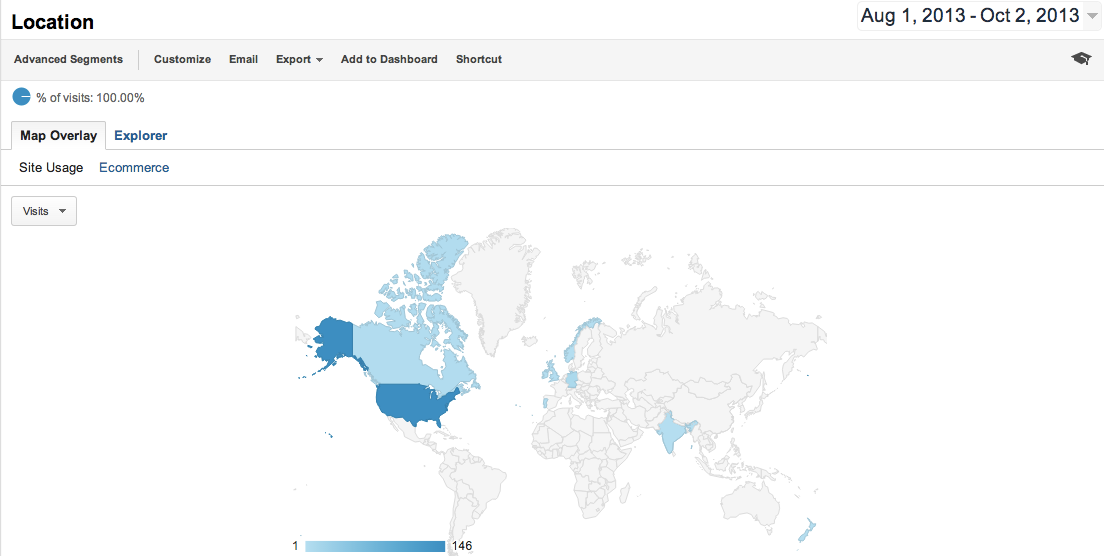
\includegraphics[width=\linewidth]{cmdmaps_location.png}
\caption{Locations of study participants}
\end{figure}
\begin{figure}
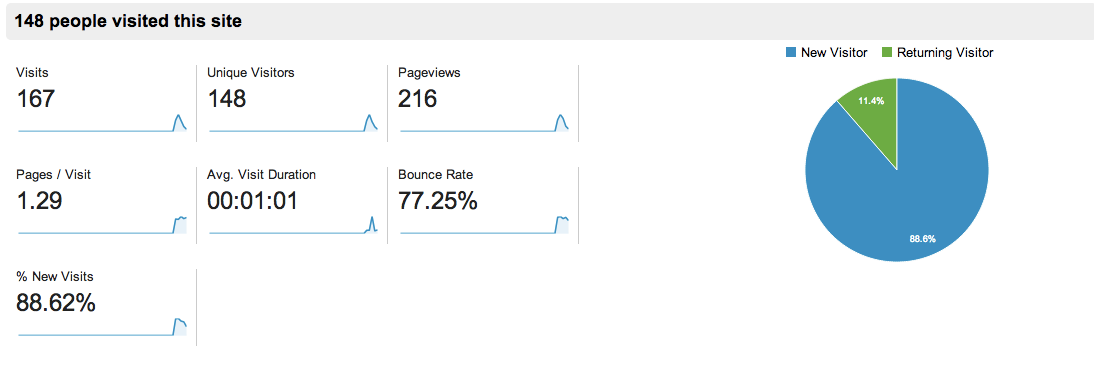
\includegraphics[width=\linewidth]{cmdmaps_stats.png} 
\caption{Website traffic statistics}
\end{figure}

To ensure that our users had the sound turned on for maximum scariness at the end, we claimed that the study was an examination of the effect of music on concentration.
\begin{figure}
\centering
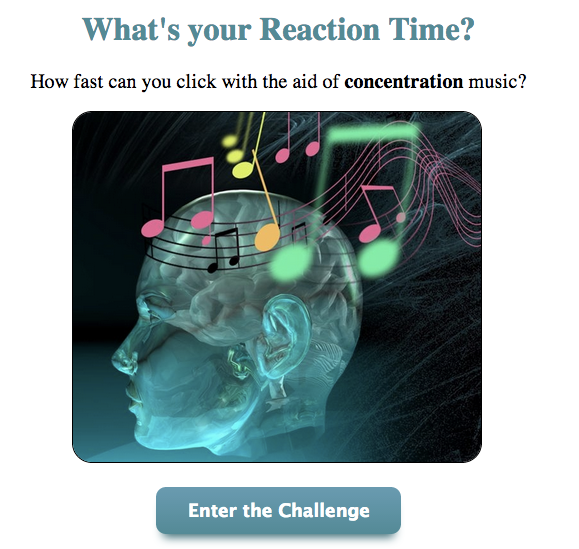
\includegraphics[width=.5\linewidth]{frontpage.png} 
\caption{The first page of our website}
\end{figure}
Once they had completed the study, we offered them a link to share the website on Facebook to give their friends a similar fright.

\begin{figure}
\centering
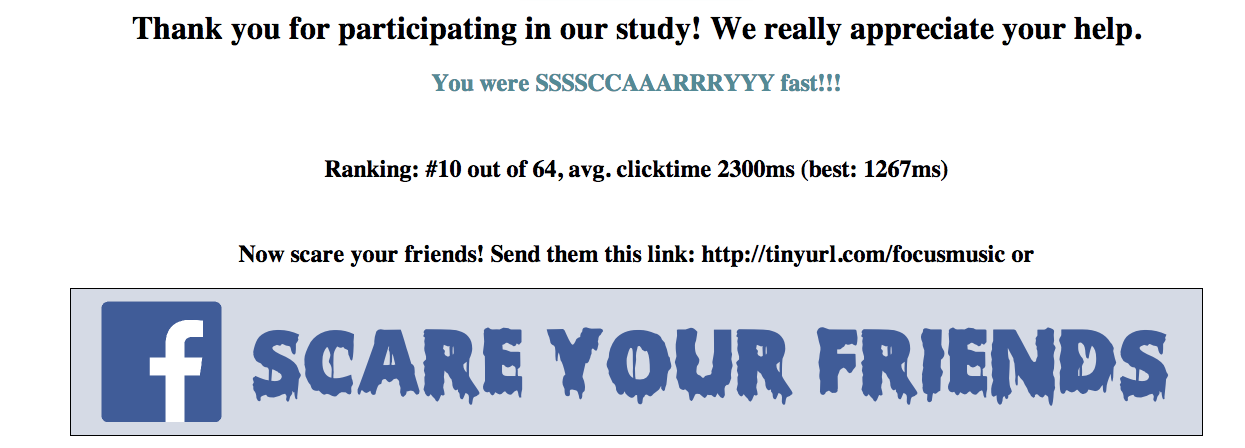
\includegraphics[width=\linewidth]{finish.png} 
\caption{The last page of our website}
\end{figure}



\end{document}